\documentclass[11pt,a4paper]{article} 


\setcounter{secnumdepth}{3}
\usepackage[T1]{fontenc}
\usepackage[utf8]{inputenc}
\usepackage{lmodern}
\usepackage{pdflscape}
\usepackage{lipsum}
\usepackage{graphicx}
\usepackage{caption}
\usepackage[font=footnotesize]{caption}
\usepackage{apacite}
\usepackage{color}
\usepackage{amsmath}
\usepackage[margin=1.5in]{geometry}
\usepackage{booktabs} 
\usepackage{xcolor}
\usepackage{float}
\usepackage{array}
\usepackage{setspace}
	\doublespacing

\date{}
\title{\huge{bleh}}

\begin{document}
\maketitle


\section{Introduction} 

In Chapter \textcolor{red}{x}, we conducted two experiments to probe the robustness of the attraction effect with complex, naturalistic stimuli. This research question arose from the debate on the real-world relevance of the attraction effect, which started with \citeauthor{Frederick2014a}'s study that described numerous failed replication attempts where the choice options were naturalistic objects. They drew the conclusion that the attraction effect is only present in choice settings where the options have numerical attributes. The findings from our experiments confirmed \citeauthor{Frederick2014a}'s results in that we have not found any evidence for the attraction effect using movies posters as stimuli.

However, as discussed in Chapter \textcolor{red}{x}, there is substantial evidence that the attraction effect is \textit{not} restricted to choice settings where the options have numerical attributes. In value-based decision making, \citeNP{Farmer2017} have demonstrated the attraction effect using perceptual representation of gambles. In one version, they adopted \citeauthor{Trueblood2013}'s rectangles to represent the probability and the nominal amount to be win (therefore, the area of each rectangle corresponded to the expected value of the gamble). In another experiment, the probability of the gamble was represented by the proportion of randomly distributed coloured squares in a 10x10 grid, whereas the nominal amount was represented as the proportion of coloured squares in another 10x10 grid. 

While these perceptual tasks are clear departures from the commonly used numerical attributes format, they are still very similar to it in one respect. Specifically, the two attribute dimensions are spatially separated and thus can be attended independently in both versions. We argue that this stimuli characteristic can be key in explaining why the attraction is so elusive in some choice contexts.

\subsection{Integral and separate dimensions} 

The idea that multiattribute stimuli can be classified based on the perceived "separability" of the attribute dimensions first arose from research focusing on similarity judgements using the method of multidimensional scaling (MDS). In essence, MDS can be used to build a low-dimensional geometrical representation of the perceived similarity between pairs of objects \cite{Hout2013}. In this representation, the objects are points in a Cartesian coordinate system and the distance between them corresponds to their perceived similarity (so that more similar objects are closer to each other). This distance can be calculated in various ways of which the Euclidean distance metric, $\delta = \sqrt{\delta_x^2 + \delta_y^2} $ is the most intuitive and well-known and was consequently used in the first applications of MDS to similarity judgements.

\citeA{Attneave1950} was the first to challenge the appropriacy of the Euclidean distance metric. He proposed that an alternative distance measure, the city-block metric, $\delta = \delta_x + \delta_y $ provides a much better fit for the similarity judgements he collected in his experiments, where he used parallelograms, squares and triangles with varying dimensions including size, tilt, and colour. According to the city-block metric, the perceived overall distance is simply the sum of the distances along the attribute dimensions.  

In contrast with \citeauthor{Attneave1950}'s results, \citeA{Torgerson1958} have found strong support for the Euclidean metric in an experiment where participants were asked to provide similarity judgements for Munsell colour chips that differed in brightness and saturation. These puzzling results led researchers to examine how the perceived similarity of objects depends on its attribute characteristics. 

In fact, the two distance metrics reflect two fundamentally different ways of perceiving object similarity. In particular, the Euclidean distance metric is invariant to axis rotation while the city-block metric is not. This means that objects whose pairwise similarity can be best described by the city-block metric have "privileged" psychological dimensions, whereas the Euclidean metric is more appropriate for objects that are processed "holistically", where the underlying attribute dimensions may not even be perceived separately \cite{Shepp1989}. 

\citeA{Shepard1964} argued that these differences can be captured by how participants justify their similarity judgements for these two classes of stimuli. For example, when the attributes can be perceived independently (stimuli that he called \textit{analyzable}), participants almost always refer to the distinct attribute dimensions when describing differences. However, in the case of stimuli that are processed holistically (for dimensions he called \textit{unitary}), they usually describe the difference along one, "combined" dimension, showing that the two attribute dimensions cannot be perceived separately. 

\citeA{Lockhead1966} investigated how the effect of dimensional redundancy differs for stimuli with \textit{separable} and \textit{integral} dimensions (these are the equivalents of \textit{analyzable} and \textit{unitary} in \citeauthor{Shepard1964}'s terminology, respectively). A redundancy gain is said to occur when performance in a selective attention task (most typically discrimination, detection, or categorization) is improved (faster and/or more accurate responses) when the two attribute dimensions vary in a correlated manner. Previous research have found redundancy gains for integral dimensions (Munsell color chips; \citeNP{EriksenHake1955}) but not for separable dimensions (visual positions of X's and O's; \citeNP{GarnerLee1962}). \citeauthor{Lockhead1966} argued that the redundancy gain stems form the fact that integral attributes cannot be attended separately, and that this concept should be key to the definition of integral attributes. 

\citeA{GarnerFelfoldy1970} have demonstrated that integral dimensions give rise to redundancy gains and interference effects using the same task. Interference effects  (slower and less accurate responses) can be observed if the two integral dimensions are orthogonal (vary in an uncorrelated manner). They concluded that dimensional integrality should be defined as those which are (1) best described by an Euclidean distance metric, (2) produce redundancy gains if the dimensions vary in a correlated fashion, and (3) show interference effects when the two dimensions are orthogonal.

More recent research have focused on how the processing of these two classes of stimuli differ. 



\textcolor{red}{research into processing of integral/separable dimensions (serial, parallel, coactive processing - Little) }

\textcolor{red}{link this with accumulator model explanations of the attraction effect (?)}

If serial processing of attribute dimensions underlies the attraction effect, then we  would only expect to see the attraction effect when the attribute dimensions are separable, but not when they are integral and cannot be attended separately. We designed an experiment that aimed to test this hypothesis.


\subsection{Method}

\textcolor{red}{broad description of the method - using two presentation formats to probe the effect - we expect to see it in the numerical version but not in the pictorial}

\subsection{Stimuli}


\textcolor{red}{refer back to integral/separable stuff and introduce the idea of using brightness and intensity as the two attribute dimensions}


In the pictorial version, we manipulated the colour (specifically, the intensity and brightness of the colour) of each teapot. In the numerical version, we used the actual numerical brightness and intensity values of the teapots. In both versions, each teapot had an underlying nominal value that was determined by its intensity and brightness, and participants learnt to infer the value of each teapot in a practice stage that always preceded the choice stage. 

\subsubsection{Choice triplet selection process}


Previous research has shown that one unit change in brightness is perceptually equivalent to a two units change in intensity \textcolor{red} {(references)}, and we took this into account when constructing the rule that determines the value of each option. Specifically, this relationship is reflected by the the red line on Figure \ref{fig:explain}, which is given by the equation
\begin{equation} \label{eq:redline}
 f_{x} = 0.5x + 0.25.
\end{equation}


\begin{figure}
\centering
\caption{Illustration of the choice triplet selection process.}
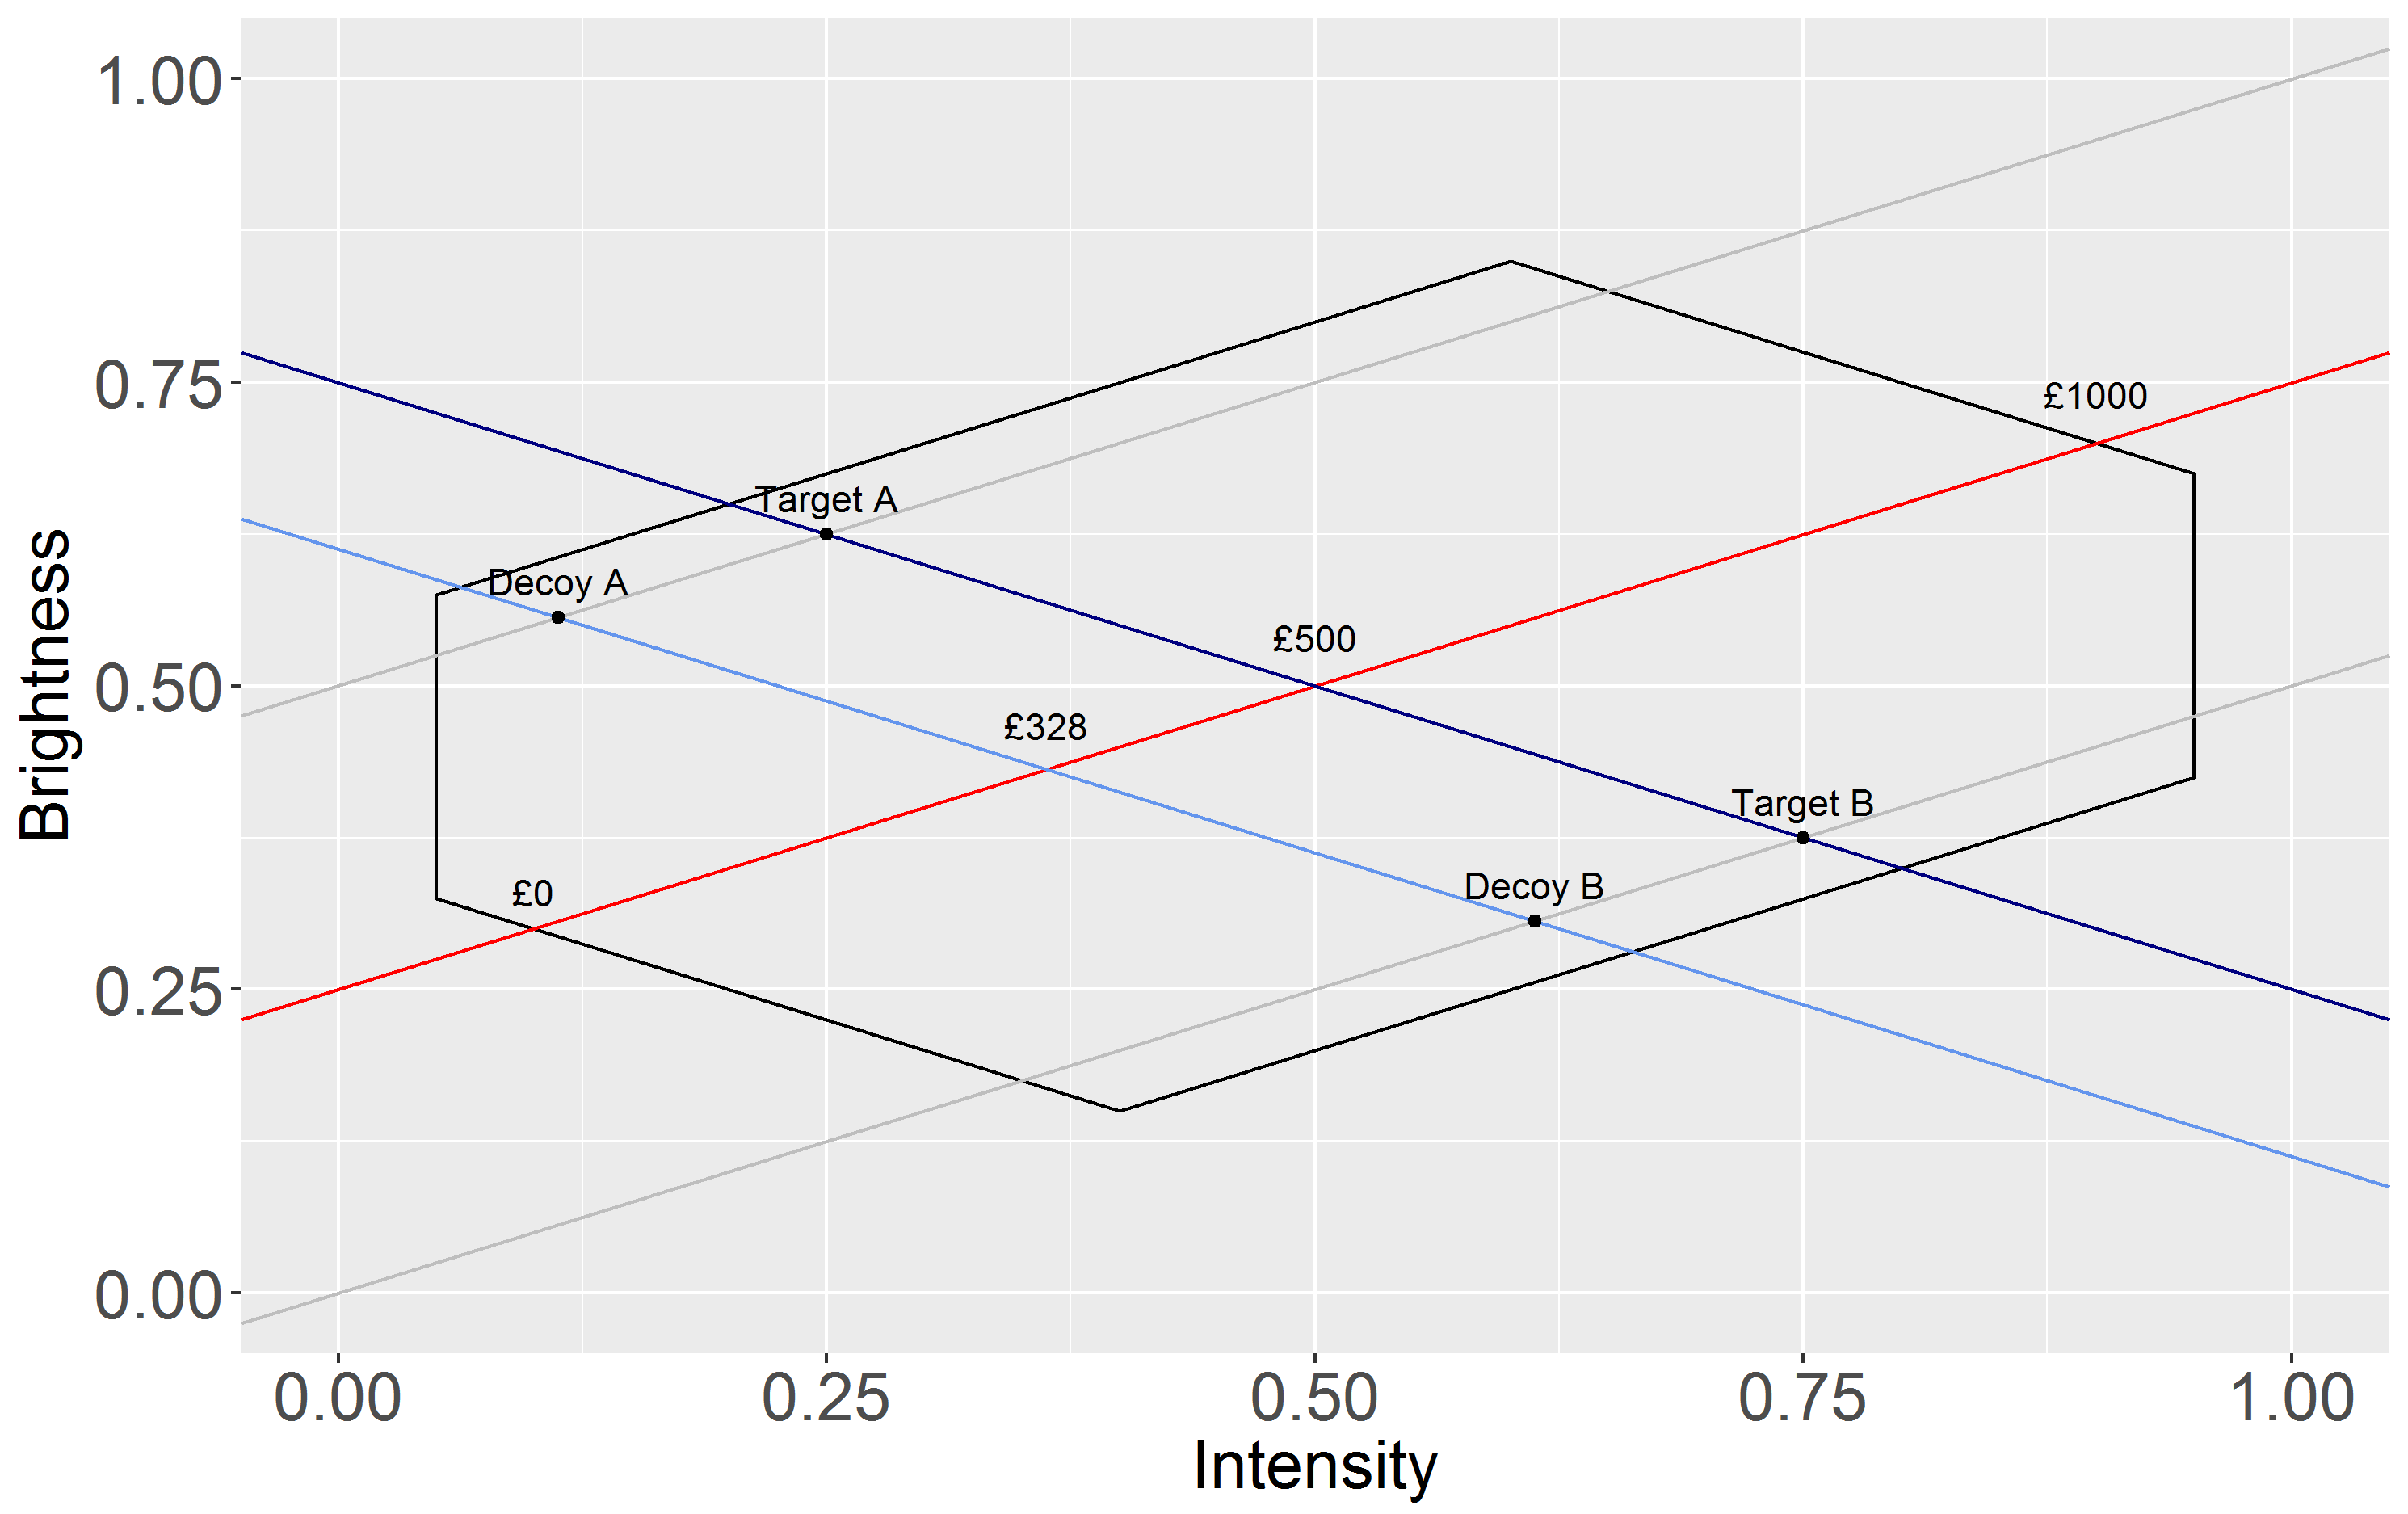
\includegraphics[width=1\textwidth]{Figure_1poly.png}
\label{fig:explain}
\end{figure}


All stimuli were required to fall within the boundaries of the black polygon displayed on Figure \ref{fig:explain}. The shape of the polygon ensured that intensity and brightness were restricted to fall between 0.05 and 0.95 and 0.15 and 0.85, respectively, which was necessary to avoid extreme attribute values that hinders the perception of the other attribute dimension (e.g., a very low brightness would translate into a black colour, regardless of the intensity value). 

 To obtain the two target candidate options, we first randomly chose a constant that was substituted into the following equation:
\begin{equation} \label{eq:blueline}
 f_{x} = -0.5x + constant,
\end{equation}
which gave us a reflection of the red line described by Equation \ref{eq:redline}, through a randomly chosen point along the same line (this point is uniquely determined by the constant and the constant was chosen so that the point always fell in the polygon). On Figure \ref{fig:explain}, this is the point where the red and the dark blue line cross, and the dark blue line is thus the reflection of the red line.

 We first created the two target candidates by selecting two points along the reflection line, one in the upper halve of the polygon (target candidate A), and another in the lower halve (target candidate B), such that the distance between the two points had to be at least half the overall length of the dark blue line within the polygon. This was important in order to ensure that one of the target candidates has a high intensity and a low brightness value and vice versa, so that they will be perceived as markedly different by the decision maker (as is required from the target and the competitor in an attraction effect choice scenario). Having created the two target candidates, the next step in creating the choice triplets was to determine the position of the decoy option. 

To create the decoy, we first randomly decided which target candidate will be assigned a decoy option. We then again reflected the dark blue line through the chosen target option (either Target A or Target B on the figure), which gave us one of the grey lines, which is parallel to the original red line. Naturally, any option along this line that lies to the left of the target will be inferior to it. 

However, all decoys need to satisfy two criteria. First, a decoy needs to be sufficiently far away from the target option, so that the dominance relationship can be easily identified. Perceiving the dominance relationship is especially problematic with naturalistic stimuli (as opposed to a choice scenario with numerical attributes where it can be identified with absolute certainty - provided that the decision maker pays attention to the task). Therefore, we considered this criterion as the most important when creating the decoys. Second, a decoy cannot be too far away from the target, as they need to be somewhat similar to invoke an attraction effect choice situation.

Taking these into account, we decided that the decoy's position should depend on the distance between the target and the competitor (as this can vary to an extent). This avoids possible situations where the decoy is also dominated by the competitor (this can happen if the target and the competitor are relatively close, while the target and the decoy are relatively far away from each other). Specifically, we decided that the distance between the target and the decoy along the brightness dimension (y axis) should be the 27.5\% of the overall difference between the target and the competitor along the same axis. This criterion uniquely defines a point along the grey line (as shown on Figure \ref{fig:explain}).

Once we have decided on the choice triplet, the next step was to determine the value of the options. We assigned a nominal value to every point along the red line, starting with £0 and going up to £1000 (in the bottom left and top right corner, respectively, where the line crosses the polygon boundaries). Then, we could determine the value of any target, competitor and decoy within the polygon, by reflecting the red line through these points and calculate the value at the point where the two lines cross. 

For example, since the dark blue line crosses the red line at exactly halfway through its length within the polygon, the target and competitor were assigned a value of £500. Then, once we calculated the position of the decoy, we were able to construct a reflection of the red line through the decoy (the light blue line), which crosses the red line at a value of £328. Using the method described above, we generated 500 choice triplets with target, competitor and decoy, as shown on Figure \ref{fig:choice_sets}. 

\subsubsection{Experimental procedure}

In the experiment, participants were presented with triplets of teapots (with brightness and intensity attributes either represented numerically or in a pictorial fashion) and their task was to choose the teapot with the highest nominal value. Colour has three components: hue, brightness and intensity, and we fixed the hue at the value of 0.83, and varied the 
intensity and brightness that determined the value of the teapot. The experiment consisted of two parts (pictorial/numerical attribute representation). Each participant were asked to complete both parts of the experiment, and the order of the two parts was determined randomly. 


\begin{figure}
\centering
\caption{The 500 choice triplets that were used in the experiment.}
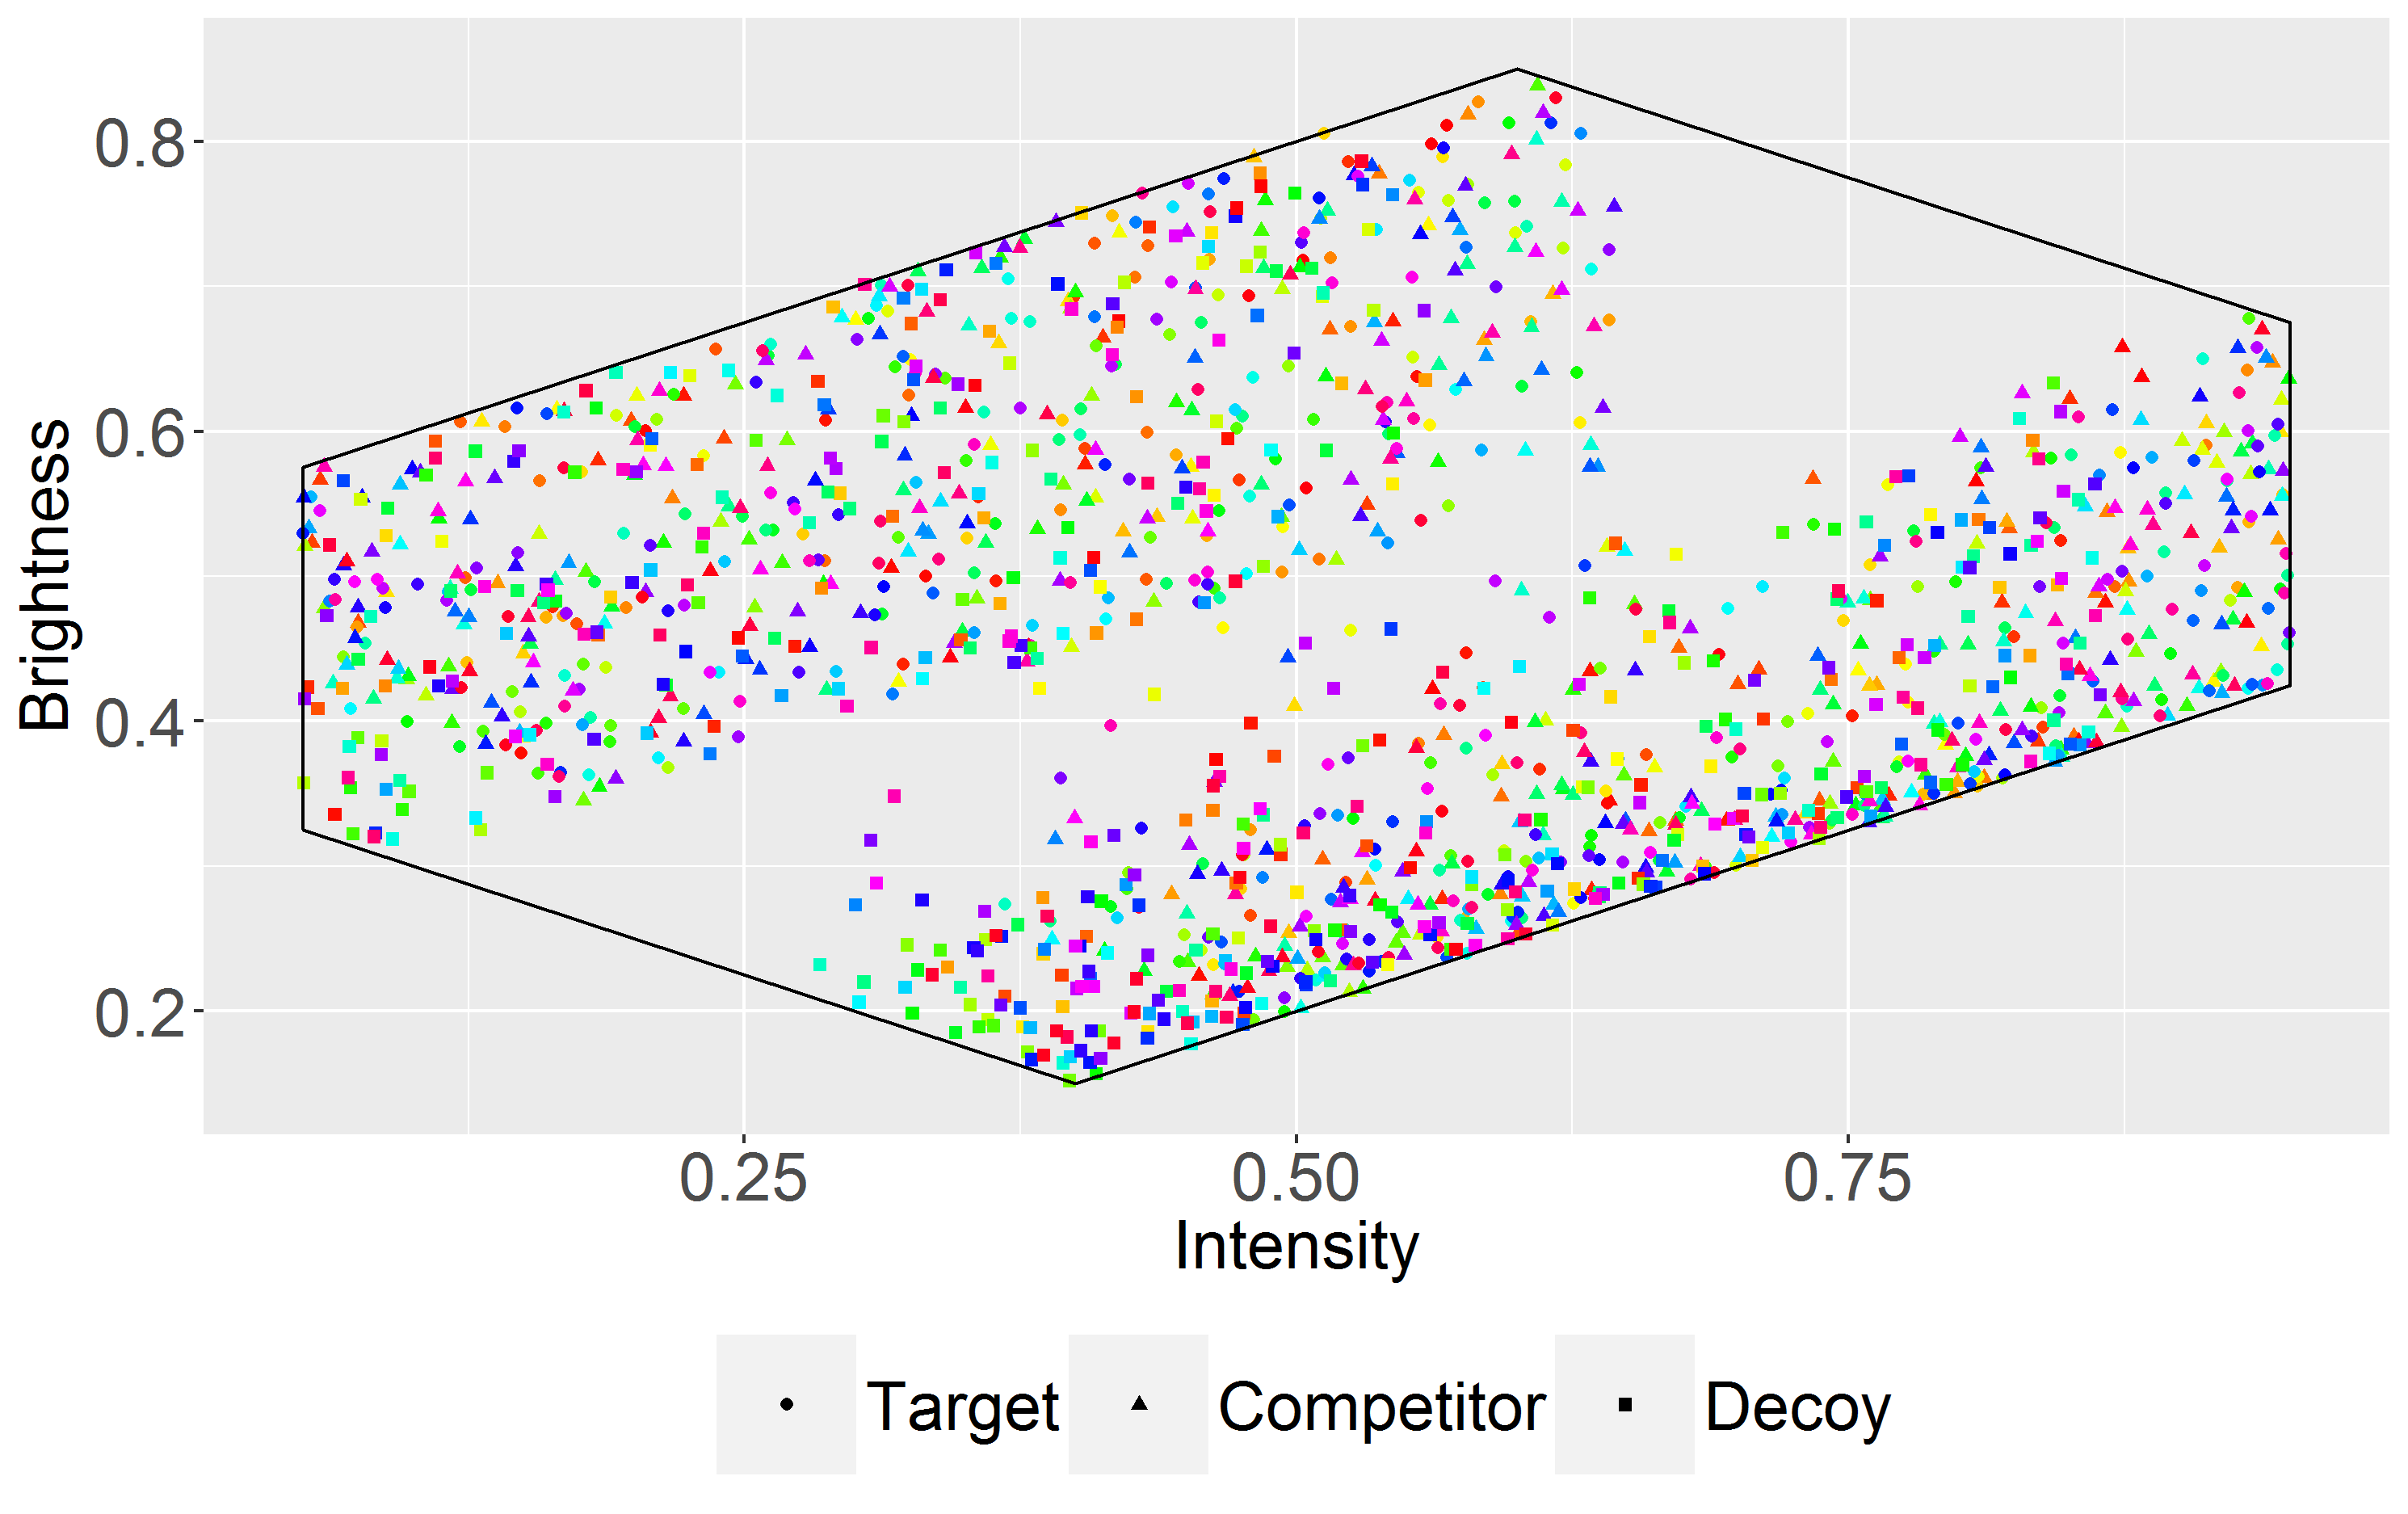
\includegraphics[width=1\textwidth]{Figure_2poly.png}
\label{fig:choice_sets}
\end{figure}

Each of the two parts consisted of two stages: a practice and a choice stage (the main task). The practice stage served to "teach" participants how to infer the nominal value of the options based on the numeric attributes/colour of the teapots. While a one-dimensional valuation rule (e.g., the brighter/more intense the colour, the better) can be fairly intuitive and thus easy to learn, when it comes to a two-dimensional learning rule, the interactions between the two integral dimensions can complicate the valuation process. To this end, each choice stage in each part was only accessible upon passing the corresponding practice stage. Before the practice stage, participants  were provided with a "valuation map" that served to explain the association between nominal value and attribute values (see Figure \ref{fig:valuemaps}). The stimuli on the valuation maps were derived from four equally spaced lines (along which nominal value is fixed) that are reflections of the red line on Figure \ref{fig:explain}.


\begin{figure}
\centering
\caption{Value maps for both choice tasks in the experiment.}
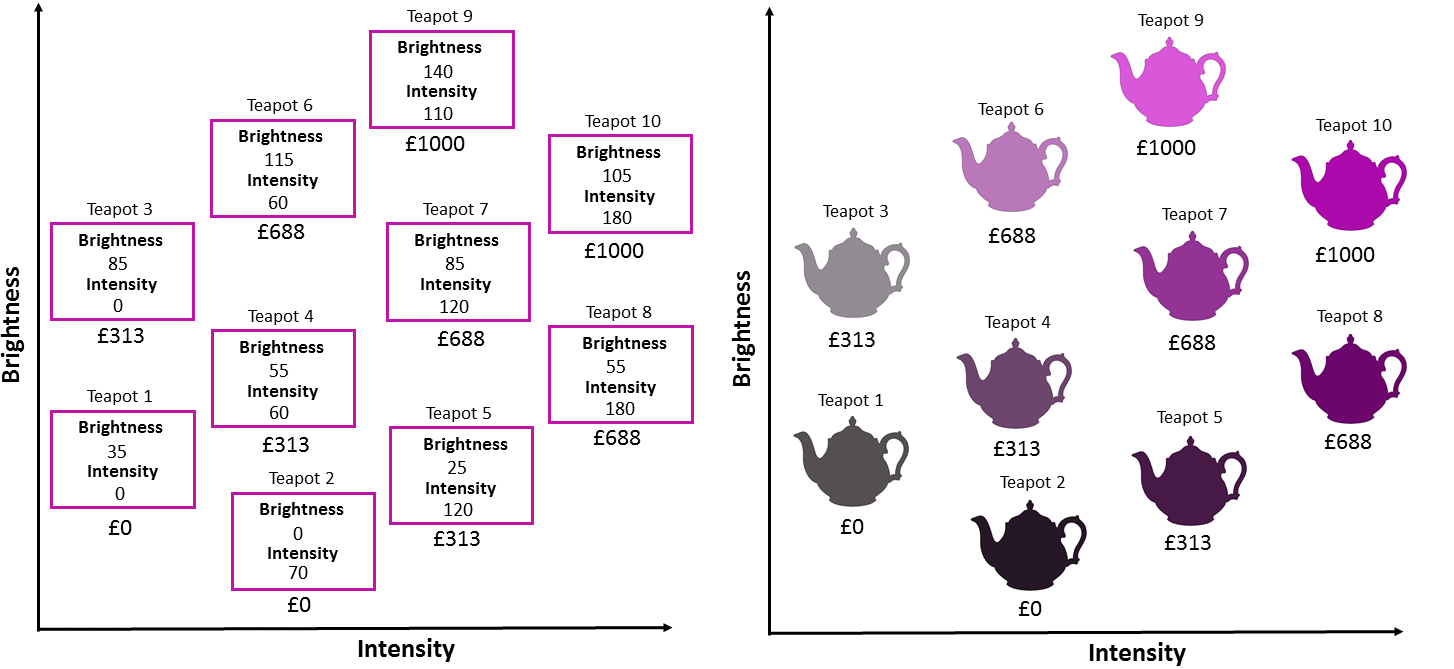
\includegraphics[width=1\textwidth]{value_maps.png}
\label{fig:valuemaps}
\end{figure}

As mentioned before, the choice triplets were generated with intensity and brightness values that ranging between 0.05 and 0.95 and 0.15 and 0.85, respectively.  We hypothesised that using integer numbers will make comparisons cognitively less demanding, therefore, in the numerical version, we transformed these values (by subtracting the minimum and multiplying it by 200), so that the new range of intensity and brightness values fell between 0 and 200 and 0 and 140, respectively. In the numerical version, we invited participants to try to infer the trade-off between the two attribute dimensions before starting the practice stage. The true trade-off is of course reflected by the red line on Figure \ref{fig:explain}: a two units change in intensity is equal to a one unit change in brightness.

Each practice stage consisted of 20 questions, where participants had to guess the relative nominal values of the two displayed options, and use the keyboard to indicate which option was worth more than the other (left/right arrow), or whether they were equally valuable (up arrow). After the keypress, participants were given feedback about whether the answer was correct, and were shown the actual nominal value of the displayed options, to facilitate learning.
In order to pass this stage and proceed to the subsequent choice task, participants had to get at least 75\% of the questions right (at least 15 questions out of 20). However, participants could attempt to complete the practice as many times as they wished, and after every failed practice session they were encouraged to consult the relevant value map. 

Using the 500 choice triplets, we created four types of practice questions, based on the value difference between the two options: equal (where the two options were of equal value), difficult (£100-£150 value difference), moderate (£150-£250 value difference), and easy (value difference higher than £250). The 20 questions in each practice session comprised of 5 questions from each type, randomly chosen from the 400 practice questions generated before the experiment (100 questions each type).


\begin{figure}
\centering
\caption{Example practice sets from types of both tasks.}
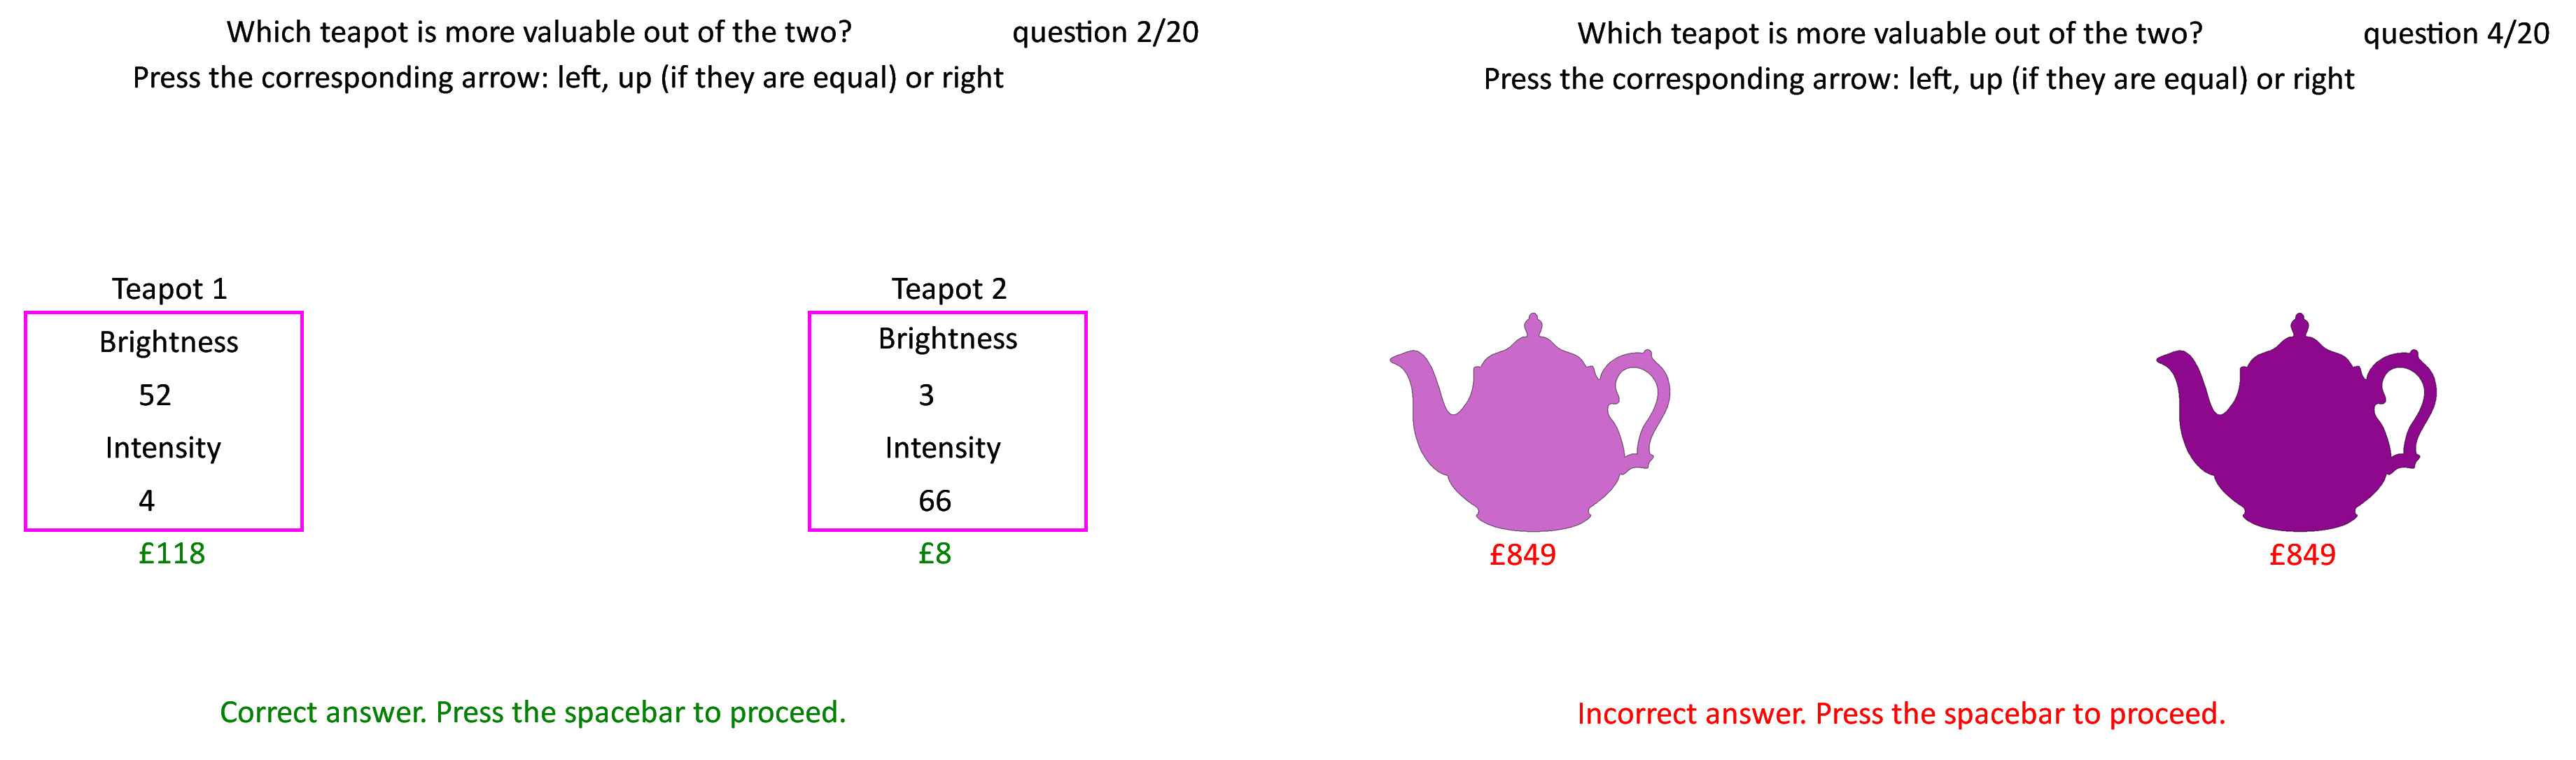
\includegraphics[width=1\textwidth]{practice.png}
\label{fig:practice}
\end{figure}


Once the participant had passed the practice stage, the choice stage began. Participants were presented with 80 choice triplets, where their task was to select the option with the highest value. Out of the 80 questions, 12 of these were catch trials that served to gauge the attention of participants. On these trials, where there was a clearly dominating option. 

To create the catch triplets (75 overall), we again used the 500 choice triplets, by first choosing an option with a nominal value of at least £300, and then two lower options that were at least worth £100 less than the high-value option. The 12 catch trials were randomly chosen from the overall 75. The rest of the trials in the choice stage were used to measure the attraction effect and were randomly selected from the 500 choice triplets (see Figure \ref{fig:choicetriplets}). During each practice and choice trial, the presentation order of the options were always randomised. Between the two parts, participants could take a break for as long as they liked.


Overall, we tested a 100 participants, all of whom were recruited through the Warwick SONA System.  We obtained ethics approval from The University of Warwick’s Humanities and Social Sciences Research Ethics Committee (reference number: 50/17-18). The study was advertised as a decision-making study, and participants were given a £4 show-up fee, and were told that they could earn £0.5 for every block of 20 correct questions, therefore, the highest possible earning in this experiment was £8 (as there were 160 questions overall). Given that the study involved completing 160 choice trials (and the two practice sessions), incentive-compatibility was important to ensure that participants stayed motivated during the choice stages. The experiment terminated after 50 minutes if the participant has not finished by then. 


\begin{figure}
\centering
\caption{Example choice triplets (from left to right: DTC and DCT).}
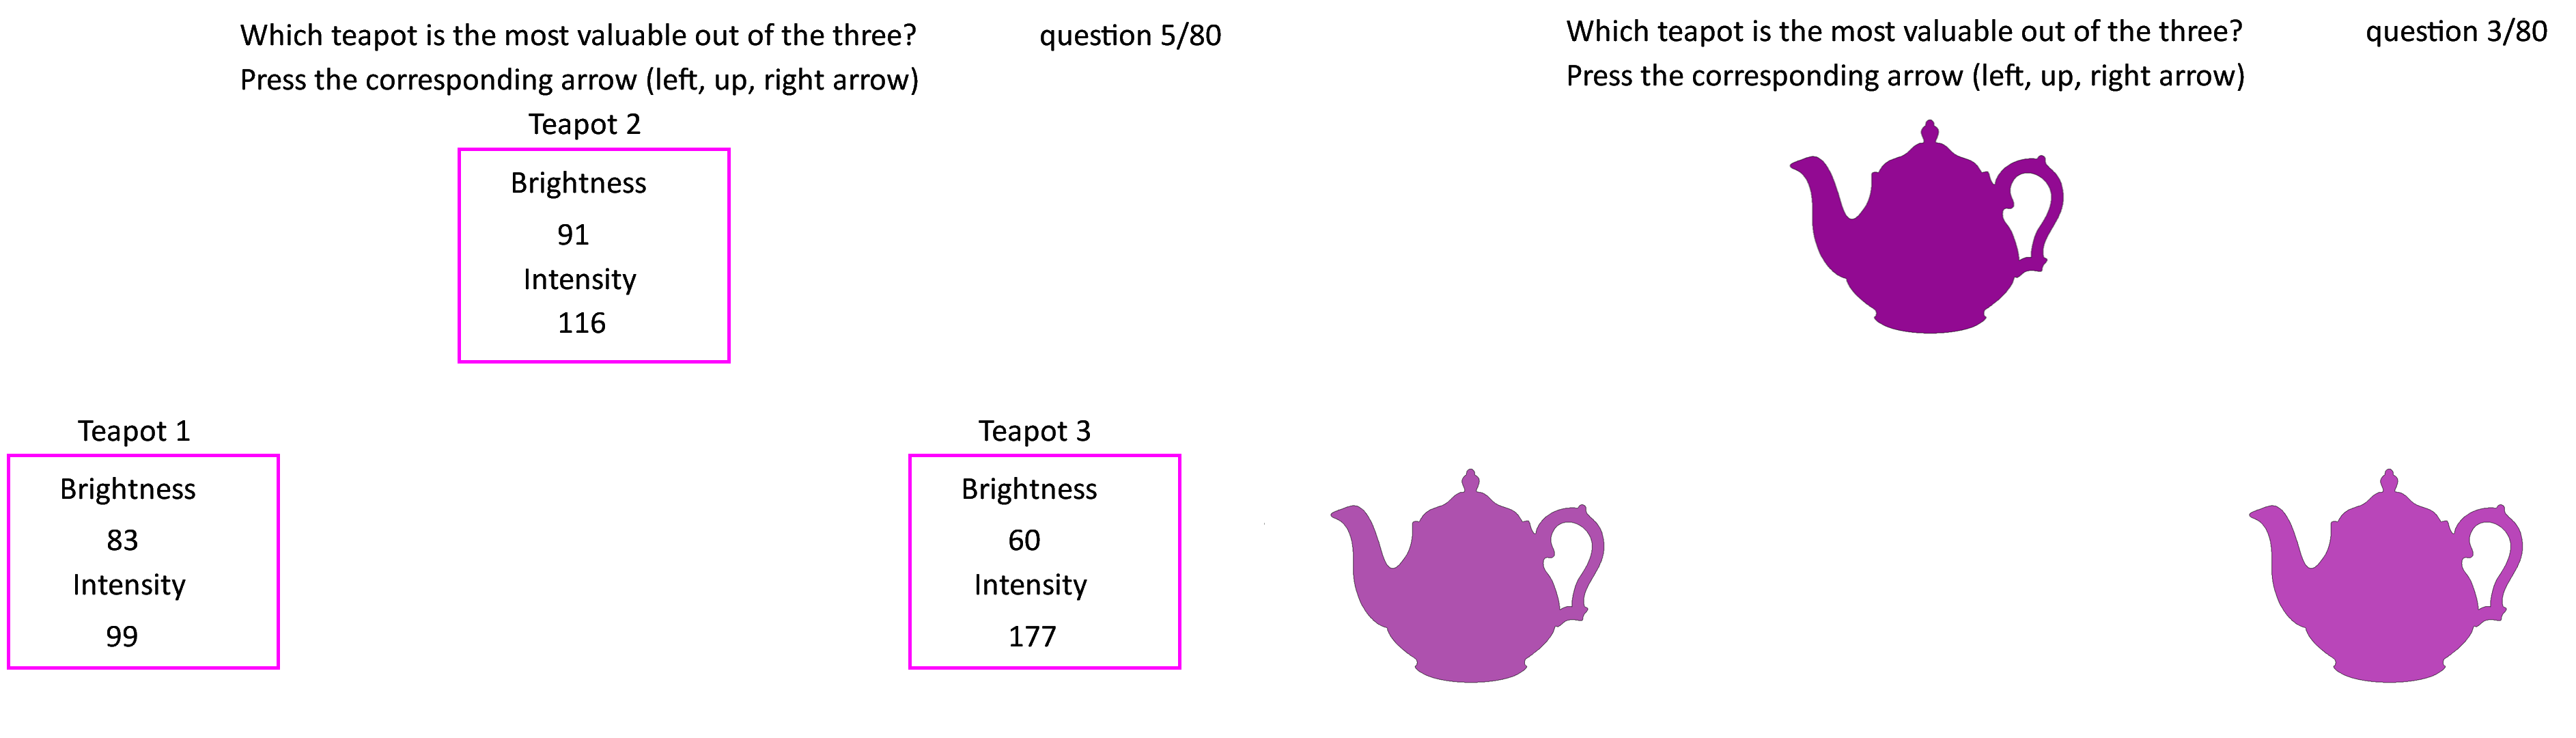
\includegraphics[width=1\textwidth]{choice_triplets.png}
\label{fig:choicetriplets}
\end{figure}


\subsubsection{Exclusion criteria}

To ensure that we only include participants who took the task seriously, we excluded choice blocks where the accuracy on the catch trials were 2.5 standard deviations below the average accuracy for that type of choice task. In addition, we excluded choice blocks that fell into the lowest 2.5\% of the entropy distribution
and the upper and lower 2.5\% of the autocorrelation distribution. Finally, we excluded trials fell into the fastest and slowest 2.5\% of
the reaction time distribution and trials where the subject selected the decoy option.
The study design, exclusion criteria and all the analyses were planned and
registered before we collected any choice data (supplement?).

\subsection{Results}

Ideally, if all of the 100 participants had completed both types of choice tasks, we would have data from 200 choice blocks (100 pictorial and 100 numerical each). However, the practice stages turned out to be more challenging for participants than we originally intended, and 14 people did not manage to pass the first practice stage in 50 minutes (or gave up earlier), and consequently we could not collect any choice data from these participants. After applying all exclusion criteria, we were left with choice data from 86 people who completed 68 pictorial and 76 numerical choice blocks. Out of the 86 people, 61 completed both the pictorial and numeric conditions.

The left panel on Figure \ref{fig:Explor_teapot} shows the number of attempts it took for participants to pass the numerical and pictorial practice stage (each attempt consisted of 20 questions, as explained above), by the order of the conditions (numerical/pictorial, therefore, there are 86 dots, each of these is a participant). This shows that for the majority of participants, it took fewer than 10 attempts to pass the practice stages, and that they found the two types of practice stages roughly equally challenging. 


\begin{figure}[ht]
\centering
\caption{Number of practice and choice trials by condition and condition order.}
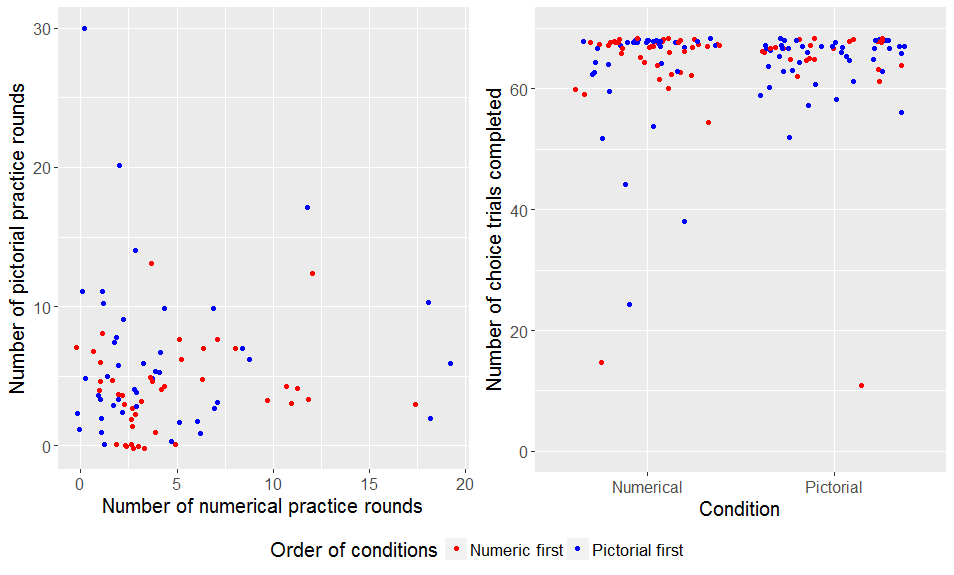
\includegraphics[width=1\textwidth]{Explor_teapot.png}
\label{fig:Explor_teapot}
\end{figure}


\begin{figure}
\centering
\caption{Proportion of trials on which the decoy was chosen by condition.}
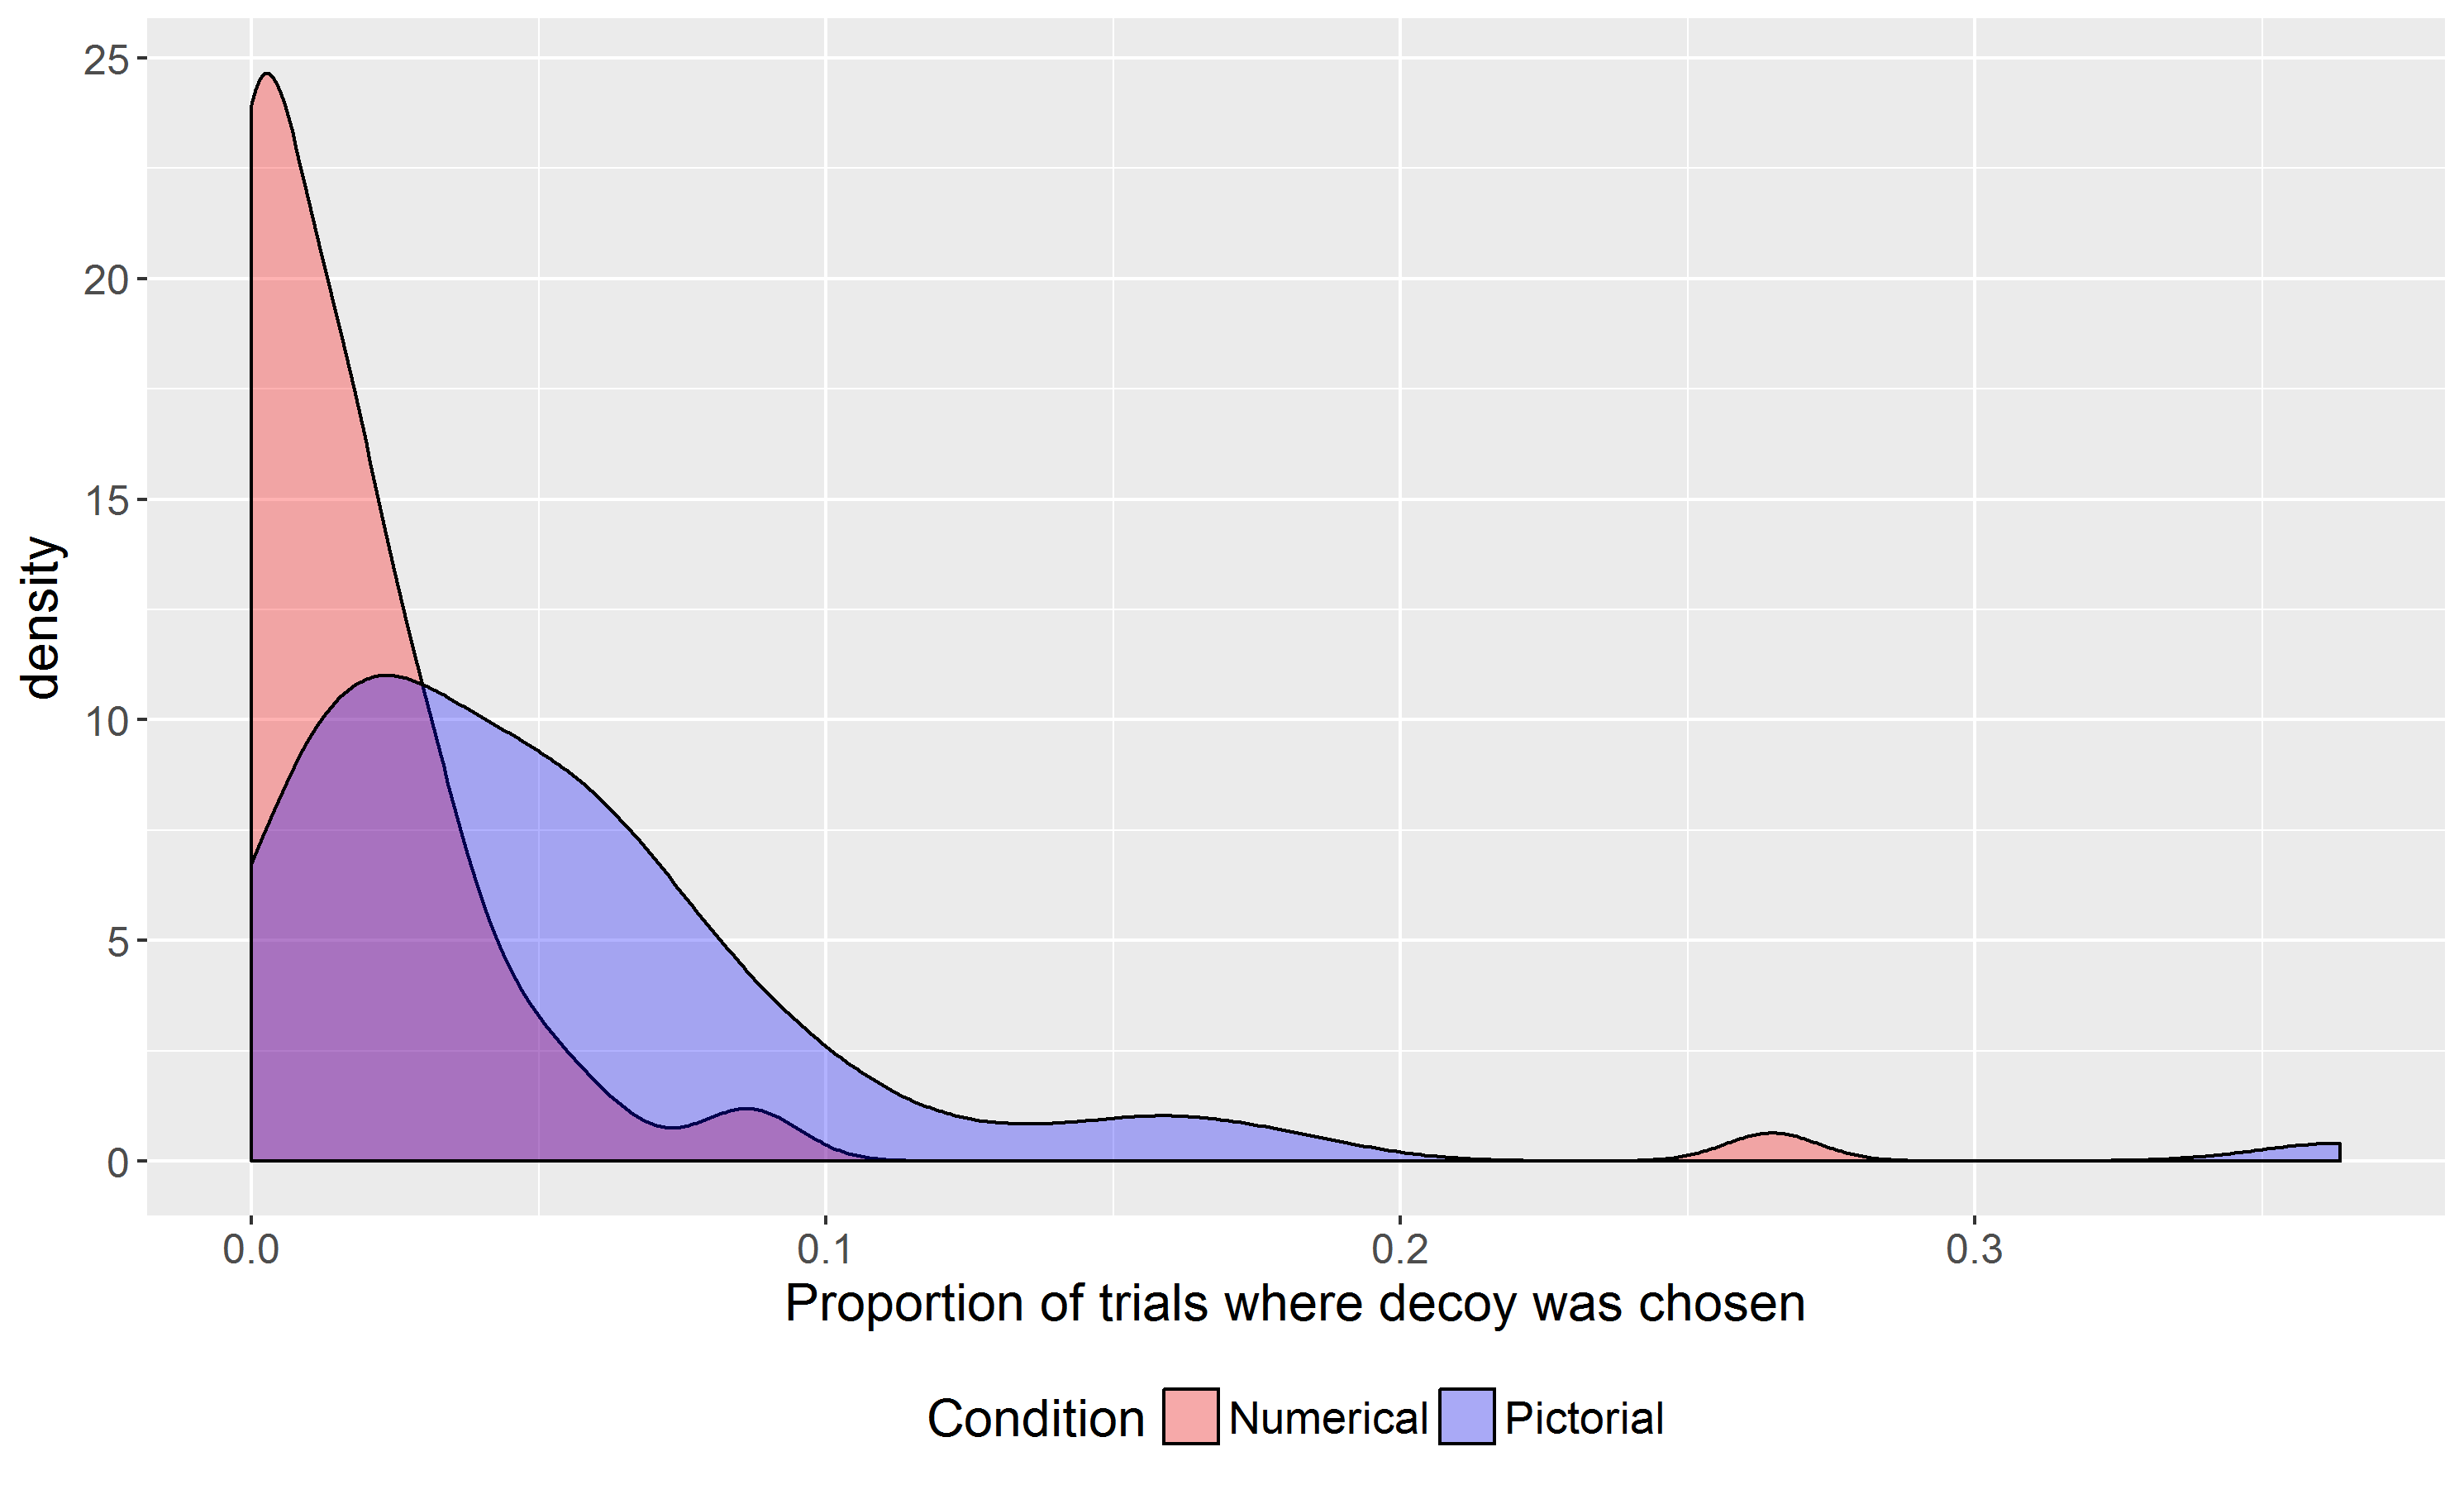
\includegraphics[width=0.8\textwidth]{Explor_teapot_dec.png}
\label{fig:Explor_teapot_dec}
\end{figure}

The right panel on Figure \ref{fig:Explor_teapot} shows the number of completed choice trials by condition and condition order (here each dot refers to a participant's condition, there are 144 of these overall). This shows that the vast majority of participants have managed to finish the choice tasks before the experiment was terminated. We also see that numerical choice stages were more likely to be interrupted, because these typically took longer to complete than the pictorial version.



Figure \ref{fig:Explor_teapot_dec} shows the distribution of the proportion of trials per condition on which the decoy was chosen. It can be seen that participants generally performed well in identifying dominated options (in 94\% of the 144 conditions, the proportion of the trials where the decoy was chosen was below 10\%). In addition, the decoy was never chosen in 45\% of the numerical and 10\% of the pictorial conditions, which indicates that participants found it much easier to identify the decoy in the numerical condition.


 \begin{figure}
\centering
\caption{Distribution of the RTs by condition, condition order and chosen item. RTs were first scaled by subject, then the median was calculated for each subject, condition, condition order and chosen item. Black points and corresponding error bars represent bootstrapped 95\% CIs of the means of these medians weighted by the number of trials.}
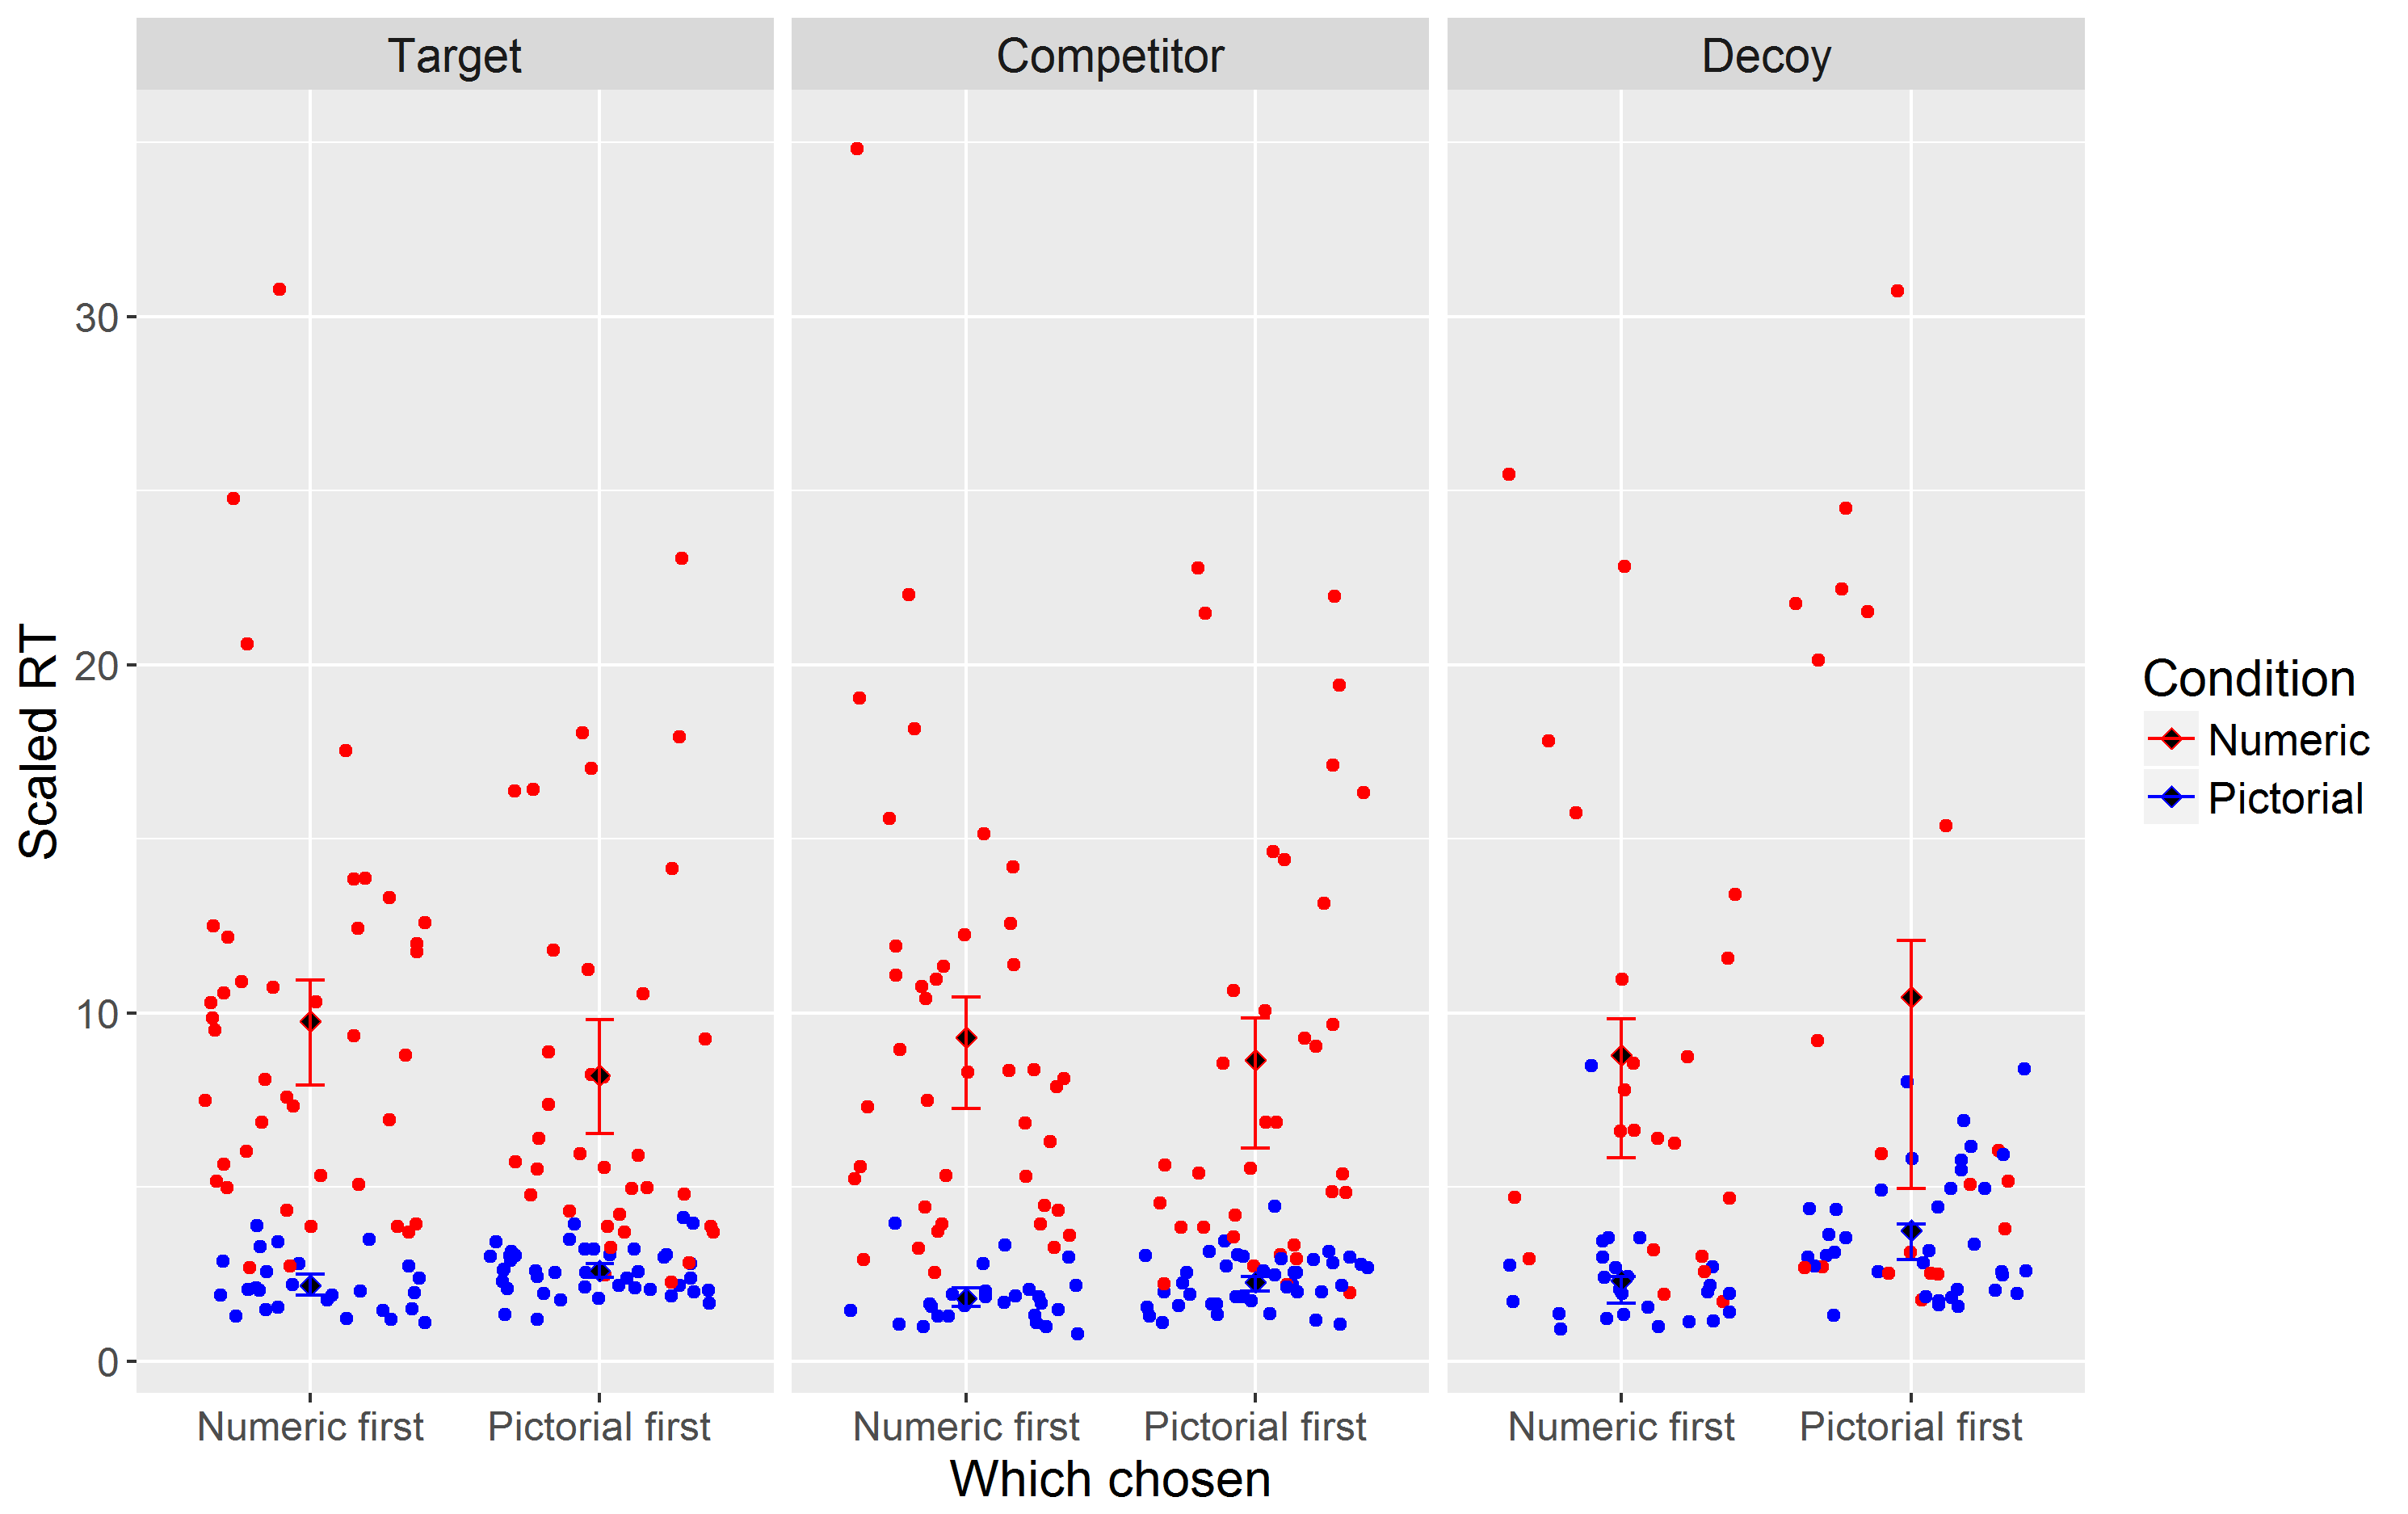
\includegraphics[width=0.8\textwidth]{Teapot_rts.png}
\label{fig:Teapot_rts}
\end{figure} 

 This is not surprising given that in the numerical version, the choice process requires the comparison of the attribute values, during which the decoy option is more likely to be identified and thus avoided, whereas in the pictorial version people are more likely to make a quicker, intuitive decision, which might result in an error. Figure \ref{fig:Teapot_rts} shows the distribution of the median RTs by condition, condition order and chosen item for each subject. As expected, participants took substantially longer to make a decision in the numerical condition. In addition, participants were generally quicker to make decisions in the condition that came second, potentially because they already knew the task or because they were slightly more tired by that point. Interestingly, we do not see differences in RTs by the chosen item. \textcolor{red} {say something about how long it took on average}

 In addition, there were no differences in the performance on the catch trials between the numerical and pictorial conditions (Wilcoxon Signed-Rank Test, p = .482, using data from the 58 participants who completed both conditions), showing that participants were equally good at spotting a dominating option in the two types of choice tasks.

As we specified in the pre-registration, to investigate how the attraction effect depends on the presentation format of the stimuli, we first tested whether the order of the conditions had any effect on the strength of the attraction effect. We calculated the attraction effect for each participant and condition, as the proportion of all trials (after excluding trials where the decoy was chosen) on which the target was chosen. The left panel on Figure \ref{fig:Teapot_condorder} shows the distribution of the proportion of trials on which the target was chosen. We can see that while the order of the conditions does not affect the strength of the attraction effect in the pictorial choice task, there is a pronounced increase in the numerical condition if it follows the pictorial choice task. We see the same result on the right panel of Figure \ref{fig:Teapot_condorder}, which shows the strength of the effect in the two choice tasks for the subset of participants who completed both types of choice tasks.   

\begin{figure}
\centering
\caption{Proportion of trials on which the decoy was chosen by condition.}
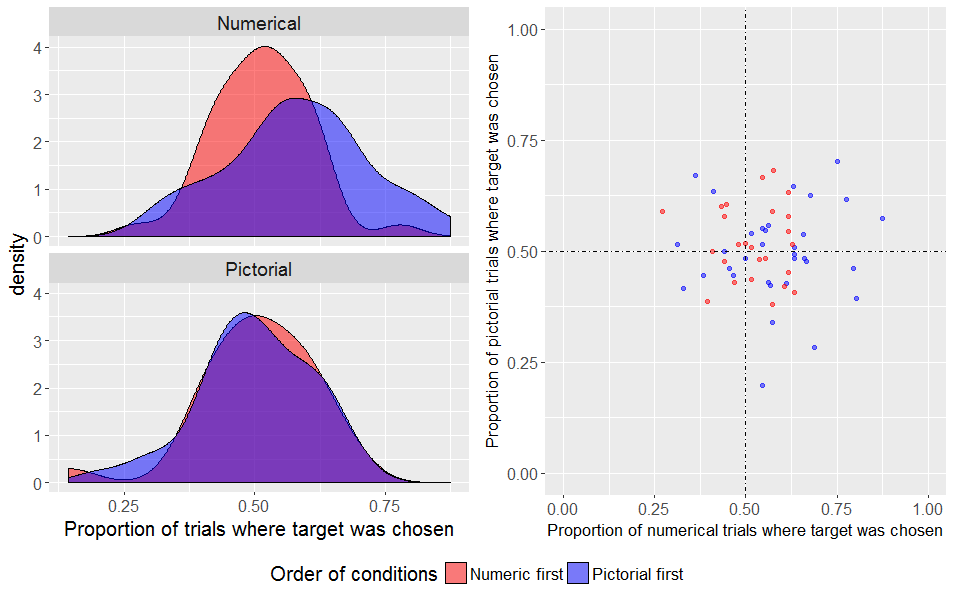
\includegraphics[width=0.8\textwidth]{Teapot_condorder.png}
\label{fig:Teapot_condorder}
\end{figure}




Table \ref{mixedeff} shows the results from a  mixed-effects logistic regression, where we predict the proportion of trials where the target was chosen with the number of practice attempts and an interaction between condition and condition order.  The results again indicate that the strength of the attraction effect in the numerical condition is much more pronounced when the first condition was pictorial. Specifically, we see a 34\% increase in the odds of choosing the target in the numerical condition, but only when it follows the pictorial condition. Interestingly, we also see a very small negative effect of the number of practice attempts: with each attempt, we see a 1.4\% decrease in the odds of choosing the target.

Since the order of the conditions modulated the effect, we only used every participant's first condition for our final test of the attraction effect. As expected from the visual inspection of Figure \ref{fig:Teapot_condorder}, when using Welch's t-test, we found no difference between the proportion of trials where the target was chosen in the pictorial (M = 0.5, 95\% CI [0.47, 0.53], N = 41) or numerical (M = 0.51, 95\% CI [0.49, 0.54], N = 42) condition, t(78.87) = 0.65, p = .52.

The strong effect of the condition order was an unexpected finding, for two reasons. First, decades of decision-making research suggests that the attraction effect is a reliable phenomenon when attribute values are displayed numerically. However, we failed to replicate this result when the numeric choice task was completed first. Even more puzzling, we see a strong effect when it follows the pictorial choice task. We can only surmise the reason for these results.

%\include{ordermixedeffects}
%\label{mixedeff}

\begin{table}[!htbp] \centering 
\captionsetup{justification=centering}
  \caption{Odds-ratios from a logistic regression (weighted by the number of trials). 95\% CIs are in brackets.} 
  \label{mixedeff} 
\begin{tabular}{@{\extracolsep{5pt}}lc} 
\\[-1.8ex]\hline 
\hline \\[-1.8ex] 
 & \multicolumn{1}{c}{\textit{Dependent variable:}} \\ 
\cline{2-2} 
\\[-1.8ex] & Target chosen proportion \\ 
\hline \\[-1.8ex] 
 Condition:Numerical & 1.000 (0.882, 1.134) \\ 
  Order:Pictorial first & 0.954 (0.840, 1.083) \\ 
  Practice attempts & 0.986$^{***}$ (0.976, 0.996) \\ 
  Condition:NumericalXOrder:Pictorial first & 1.340$^{***}$ (1.127, 1.593) \\ 
  Constant & 1.141$^{**}$ (1.024, 1.272) \\ 
 \hline \\[-1.8ex] 
Observations & 144 \\ 
Log Likelihood & $-$543.168 \\ 
Akaike Inf. Crit. & 1,096.336 \\ 
\hline 
\hline \\[-1.8ex] 
\textit{Note:}  & \multicolumn{1}{r}{$^{*}$p$<$0.1; $^{**}$p$<$0.05; $^{***}$p$<$0.01} \\ 
\end{tabular} 
\end{table} 



One obvious difference between our experimental task and the standard choice tasks used to investigate the attraction effect is that in our task, participants had to learn the underlying trade-off between the attribute values, as opposed to relying on a more intuitive, preferential valuation rule. This is problematic for two reasons. First, it means that our experimental task was conceptually different from a standard preferential choice task, as the choice process involved consulting a previously learnt rule, which is unlikely to resemble to a preferential choice process. A second, related issue is that in the practice stages, we trained participants to be experts in inferring the nominal value of the options, while it has been previously shown that the attraction effect tends to be stronger when the decision maker is unfamiliar with the choice domain, and weakens with expertise (references). 

However, even if these concerns have some validity, they do not offer a comprehensive explanation for our results. Specifically, they cannot accommodate the fact that we found a strong effect of condition order. Our results show a strong attraction effect in the numerical condition when it follows the pictorial condition, and no attraction effect when the numerical condition comes first.

We can only conjecture the underlying reason for this puzzling result. One possible explanation could be that since the numerical task required more cognitive effort, and there were many questions to be completed (80 questions in each choice task, and passing the two practice stages, which often took longer than the choice stages), participants might have spent less time deliberating and were more likely to rely on intuitive thinking when the numerical condition followed the pictorial one, which might have given rise to the attraction effect. 

However, Figure \ref{fig:Teapot_rts} shows no substantial difference between RTs in the two conditions by condition order, and Table \ref{mixedeff} indicates that the number of practice attempts has a small \textit{negative} effect on the strength of the attraction effect (as opposed to a positive effect, as we would expect if "tired" participants were more likely to choose the target).

We also tested whether the tendency to choose the target in the numerical condition that follows a pictorial condition changes over time. If participants get tired towards the end of the experiment, \textit{and} they are more susceptible to the attraction effect when tired, then we would expect that they choose the target more often towards the end of the experiment. 

To this end, we divided the number of trials in each condition into 4 equal sized blocks (in their temporal order), and calculated the corresponding target choice proportions for each blocks. If the overall number of trials were not a multiple of 4, then the remainder was allocated to the fourth block. Figure \ref{fig:Block_order} shows the average target proportion by condition, condition order and block number.

We see a slightly increasing temporal tendency to choose the target in the numerical condition if it follows the pictorial condition. While this pattern is somewhat consistent with a cognitive effort explanation, the analysis of RTs and the slight negative effect of practice trials are not consistent with this explanation. In addition, we did not collect any data on participant's cognitive engagement, and the link between susceptibility to context effects and resource depletion is at best disputed in the literature. 


\begin{figure}
\centering
\caption{Mean target choice share by condition, condition order and block number. Error bars represent 95\% bootstrapped CIs, weighted by the number of trials in each block.}
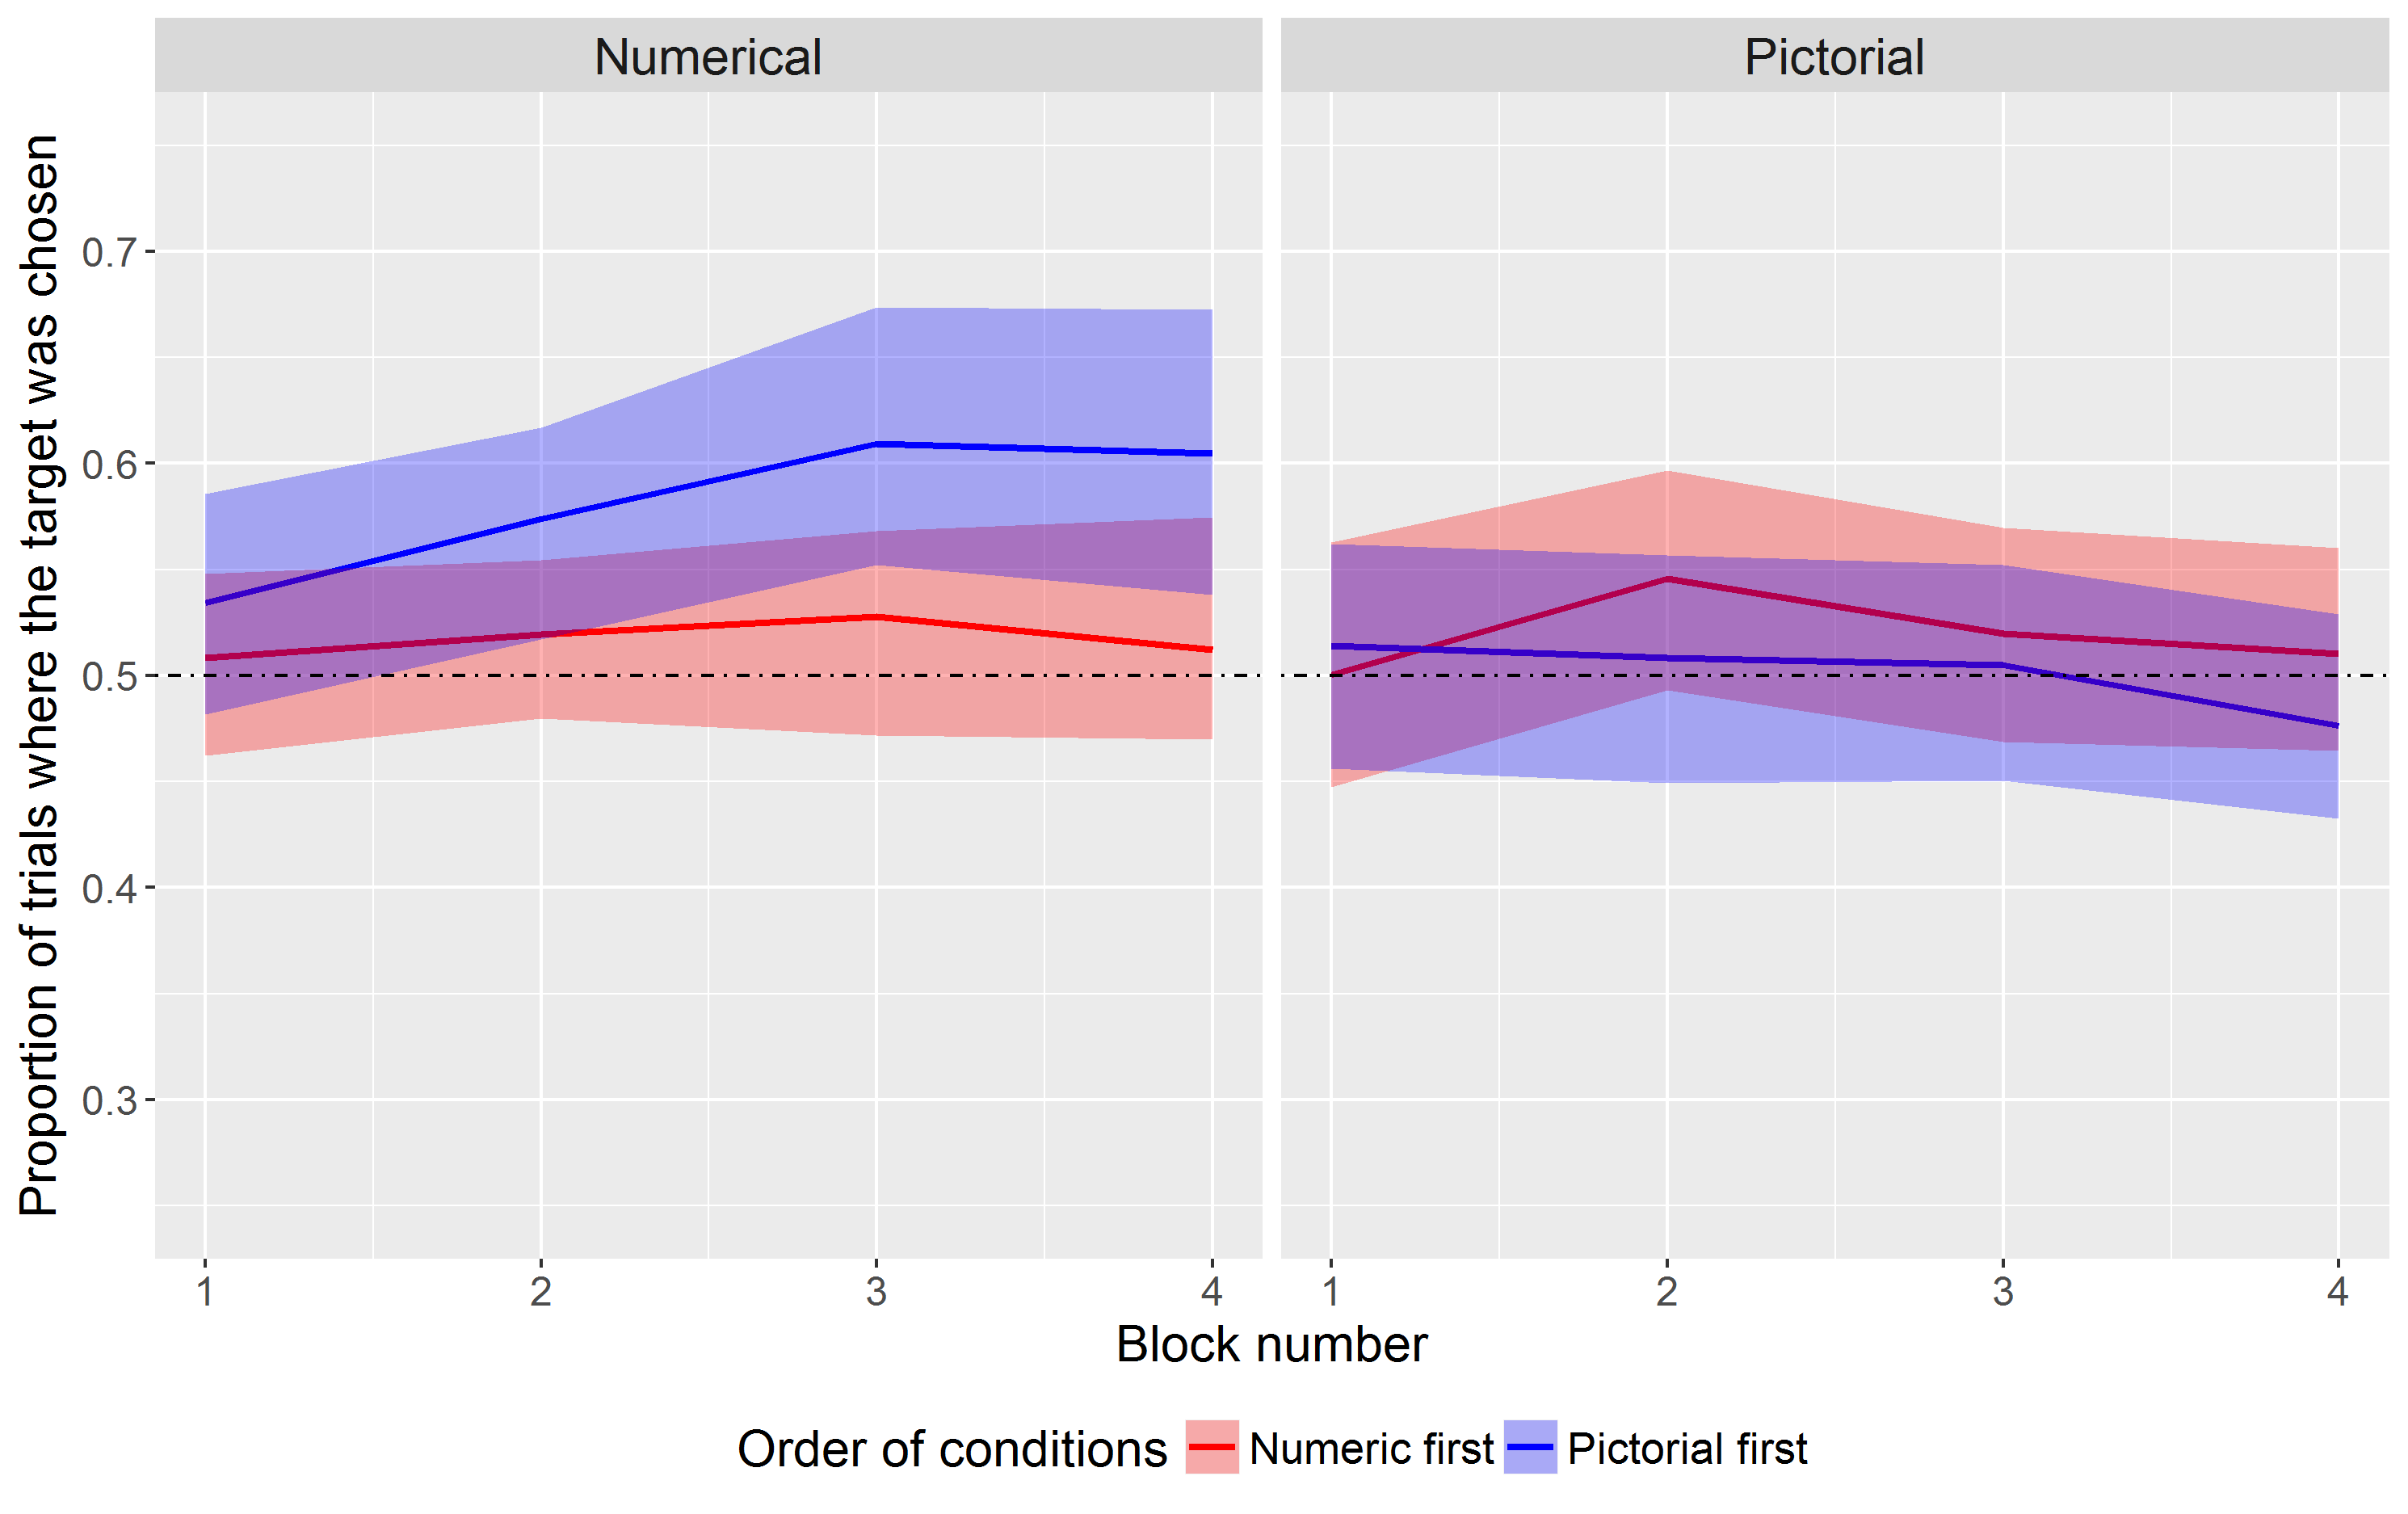
\includegraphics[width=1\textwidth]{Block_order.png}
\label{fig:Block_order}
\end{figure}




\subsection{Discussion}

This study set out to investigate how the attraction effect depends on the presentation format of the stimuli. Our earlier study had failed to replicate the effect using a complex, naturalistic stimuli, so we created a simplified, artificial stimuli that can be represented in a pictorial and numerical format to test if it is the separable nature of the attribute dimensions that gives rise to the attraction effect.  We expected to see a strong attraction effect in the numerical condition, and no attraction effect in the pictorial condition.

Somewhat unexpectedly, we found that the effect in the numerical condition depends on the order of the conditions: the attraction effect was only present in the numerical condition if it followed a pictorial condition. 

We can only speculate about the exact cognitive processes underlying this effect.

















\bibliographystyle{apacite}

\newpage

\bibliography{refs}


\end{document}